\scanpage{243}

\[
\operatorname{Pic}(X_n)\xrightarrow{\sim}\underline{\operatorname{Pic}}_{X_n/k}(k)
\]
et du th. précédent. Dans le cas général, \unsure{Notons} \deleted{d'abord} \unsure{ceci|cas} [où $k'/k$ est une extension finie de $k$, \unsure{que l'on choisit} de façon

\deleted{\uline{Lemme} Sous les conditions du corollaire [car. 0 \unsure{essentielle}, mais non la \unsure{propreté}], le conoyau de $\operatorname{Pic}(X_m)\unsure{\text{---}|\longrightarrow}\operatorname{Pic}(X_n)$ (pour $m\geq n$) est sans torsion.}

\deleted{On est \unsure{ramené} au cas où $m=n+1$, où cela \deleted{\unsure{en}} résulte du fait que ce conoyau est $\subset\mathrm H^2(X_0,\deleted{\unsure{F_2}}\inserted{F^{(n)}})$, $F_{\deleted{\unsure{n}}}^{(n)}$ un Module \unsure{coh.} convenable sur $X_0$.}

pour \deleted{\unsure{le}} $X_0\otimes_k k'$ satisfasse \unsure{aux} conditions énoncées plus haut] : on a une suite exacte

\diagram{\begin{tikzcd}[column sep=large]
0\arrow[r] & \operatorname{Pic}(X_n)\arrow[r] & \underline{\operatorname{Pic}}_{X_n/k}(k)\arrow[r] & \check{\mathrm H}^{2}(k'/k,M_n)
\end{tikzcd}}

\margin{\uline{\unsure{rigoureux}??} \quad \uline{À \unsure{expliciter}}}
\figure{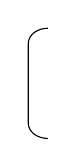
\begin{tikzpicture}[x=1cm,y=1cm]
\draw (0.25,0) to[out=180,in=-90] (0,0.2) -- (0,1.2) to[out=90,in=180] (0.25,1.4);
\end{tikzpicture}}

où $M_n$ est le schém. en groupes [comm. \unsure{lisse} connexe] \deleted{\unsure{tel}} qui décrit les unités de la $k$-algèbre \deleted{$\unsure{k_2}$} $\mathrm H^0(X_n,\mathcal O_{X_n})$. On voit que le système projectif des $(M_n)$ satisfait M.L. [groupes \deleted{alg. \unsure{connexes}}\inserted{\uline{de type fini} sur $k$ !}] et est à noyaux \deleted{\unsure{unipotents}} [\unsure{ici}, \uline{vectoriels}\ldots]

\margin{242}
